 \mychapter{Funcions i gràfics}{Funcions i gràfics}{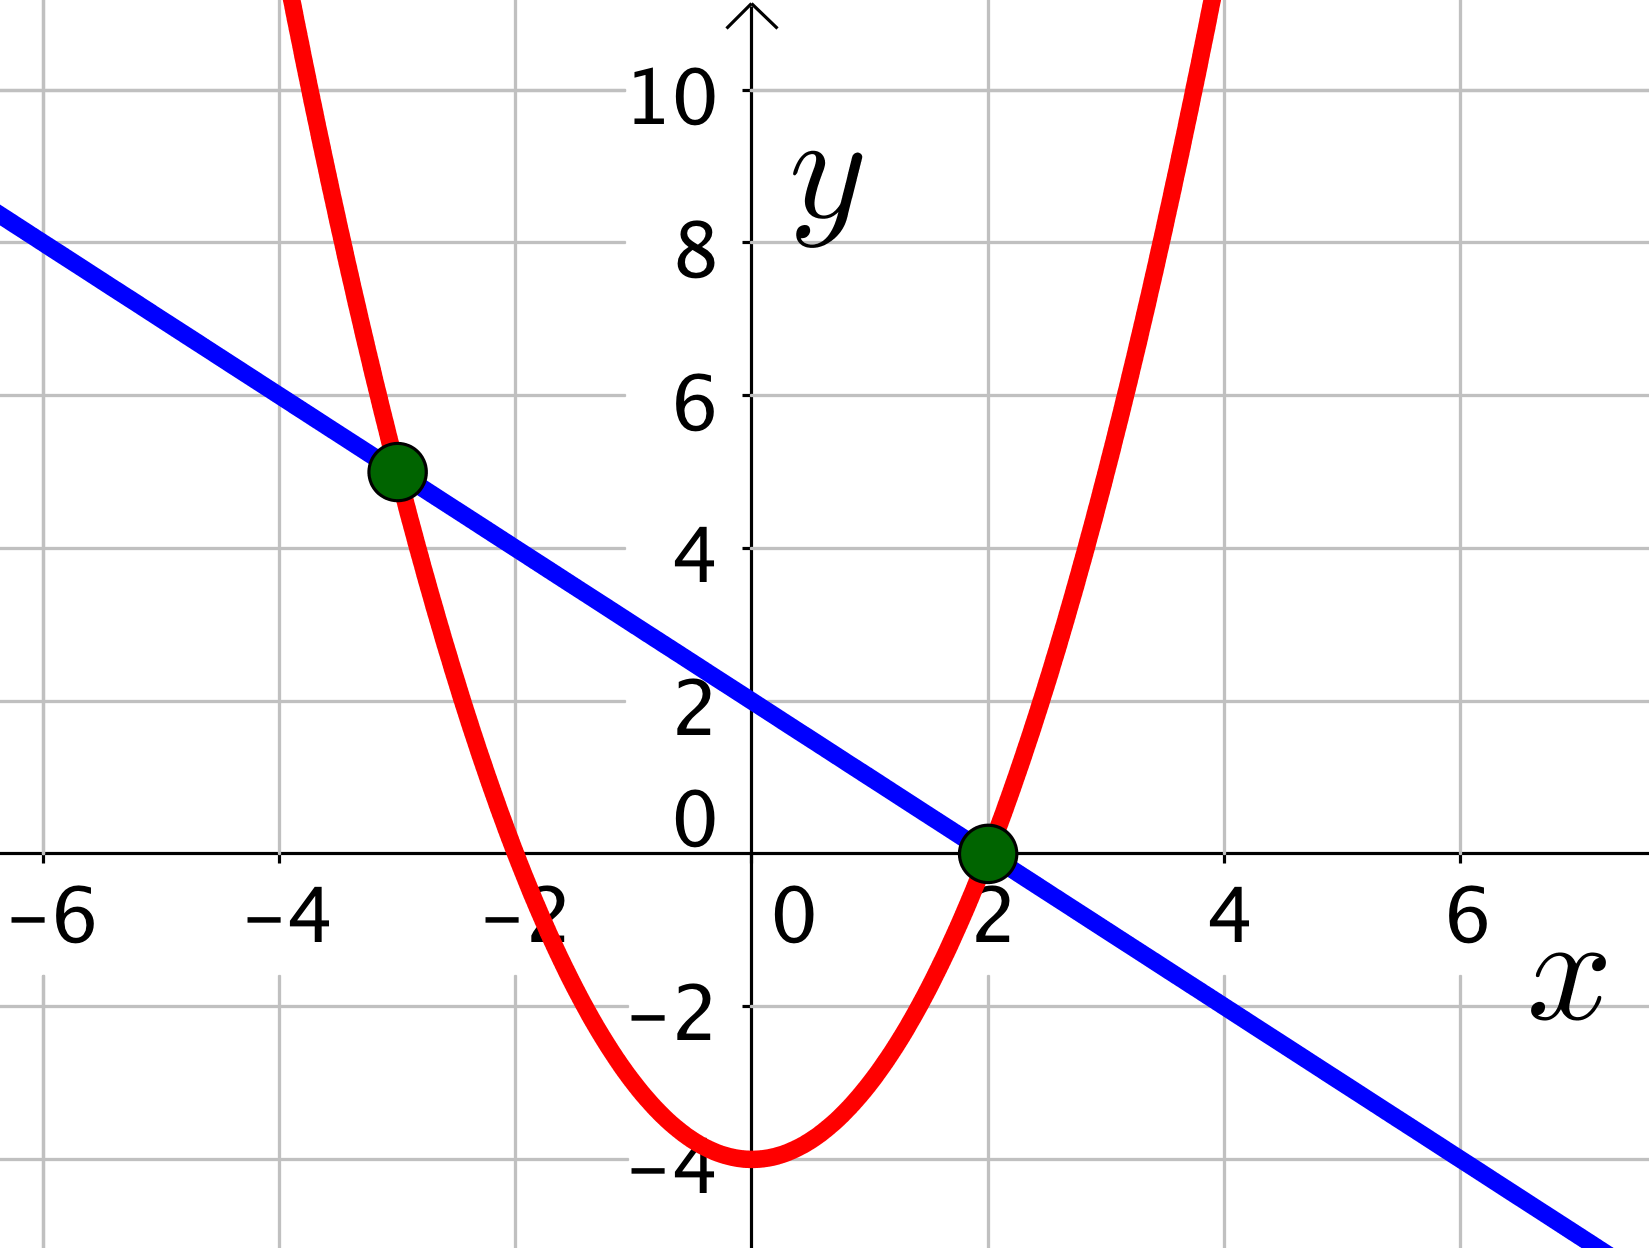
\includegraphics[width=4.5cm]{img-08/portada}}{chap:funcions}

\section{Sistemes de representació en el pla}

\begin{theorybox}

 Per representar punts en el pla utilitzam un sistema d'eixos perpendiculars (\textbf{Eixos cartesians}) que es tallen a un punt \textbf{O(0, 0)} anomenat \textbf{origen}. 
 
 L'eix horitzontal s'anomena eix de les \textbf{abscisses (eix X)}.
 	
 L'eix vertical és l'eix de les \textbf{ordenades (eix Y)}.
\end{theorybox}

 
\begin{mylist}

\begin{comment}
\exer  \includegraphics*[bb=0 0 2.75in 1.86in, width=2.75in, height=1.86in, keepaspectratio=false]{img-08/image1.png}

Fixa't en el mapa següent, localitza els països o ciutats que es demanen i indica en el teu quadern:


 a) Els quadrants on es troben els següents països:

 Mèxic:  Madagascar: Índia:  Xile:  Espanya:  Argentina:

 Austràlia: Japó: Aràbia Saudita:

 Alemanya: EUA: Marroc:

 b) Les coordenades (aproximades) de les següents ciutats:

 Ciutat del Cap: Pequín:  Londres:

 Nova York: Rabat:  Còrdova(Mèxic):

 Rio de Janeiro: Sidney:  Oviedo:   Alacant:

\end{comment}
 

\vspace{-3cm}
\exer  \begin{minipage}[t]{0.5\textwidth} a) Copia en el teu quadern i indica les coordenades de tots els punts que estan representats en el gràfic: 

 b) Representa gràficament en el teu quadern els següents punts del pla: 

\begin{tabular}{lllll}
 A(0,-2) &  B(-2,0) & C(4,0) & D(-6,0) \\
 E(0,6) & F(1,7) & G(7,1) & H(-4,8) \\
  I(-1,-4) & J(-4,-1) &  K(5,-3) &  L(9,6) \\
  % M(-2,1)  & N(7,-4) & Ñ(-3,-3) &  O(0,0) \\
  %  P(-2,-1) & Q(2,1) & R(2,-1) & S(-1,1) 
\end{tabular}

\end{minipage}
\begin{minipage}{0.5\textwidth}
	\vspace{3cm}
 \includegraphics*[width=0.9\textwidth]{img-08/punts}
\end{minipage} 


\answers{a) A(--4,2); B(--2,0); C(--3,--2); D(--1, 3); E(1,2); F(1,--1); G(3,0); H(3,4); I(4,--2); J(5,--3)}

\exer   Representa en un gràfic els punts següents, triant una escala en els eixos que permeti dibuixar-los tots de forma còmoda: \textit{A}( 5,4); \textit{B}(0,2); \textit{C}(--2,0); \textit{D}(3,--1.3); \textit{E}(1.5,0); \textit{F}(0,0); \textit{G}(--1,--2/3). Assenyala en cada cas a quin quadrant pertany el punt o, si escau, sobre quin eix està.

\vspace{2cm}
\exer  Situa en un sistema de referència cartesià els punts següents: 

A(0, 4); B(0, 2.3); C(0, --2); D(0, --1). Què tenen en comú tots ells?

\answers{Tots ells es troben sobre l'eix de les ordenades.}

\exer \mental Digues les coordenades de tres punts situats en el tercer quadrant.

\answers{Per exemple (--3, --2); (--1, --5); (--2;--2). Les dues coordenades són negatives.}

\exer  \mental Digues les coordenades de tres punts de l'eix d'ordenades. Què tenen en comú? 

\answers{Per exemple (0,3); (0,--5); (0,1). Tots tenen la primera coordenada igual a zero.}

\end{mylist}



\section{Concepte de funció}


\begin{theorybox}
\video[ytid=2v2DOKGk\_PI]{190}{Introducció a les funcions}
 Una \textbf{funció} és una \textbf{relació} entre dues variables $x$ (variable independent) i $y$ (variable dependent) de tal forma que per cada $x$ trobam un \textbf{únic} valor de $y$.

 Una funció es pot donar de diverses formes:
\begin{itemize}
	\item A través d'una gràfica 
	\item Amb un enunciat 
	\item Amb una taula de valors
	\item Amb una fórmula (expressió analítica)
\end{itemize}
\end{theorybox}


\begin{mylist}
 
\exer \mental De les següents relacions entre dues variables, raona quines són funcionals i quines no:
\begin{tasks}(1)
   \task $x:$ Edat i $y:$ altura de la persona al llarg de la seva vida \hspace{1cm} \dotfill \hspace{1cm}
   \task $x:$ Altura i $y:$ edat de la persona \hspace{1cm} \dotfill \hspace{1cm}
   \task $x:$ Preu de la gasolina i $y:$ dia del mes \hspace{1cm} \dotfill \hspace{1cm}
   \task $x:$ Dia del mes i $y:$ preu de la gasolina \hspace{1cm} \dotfill \hspace{1cm}
   \task $x:$ Un nombre i $y:$ la seva cinquena part \hspace{1cm} \dotfill \hspace{1cm}
   \task $x:$ Un nombre i $y:$ el seu quadrat \hspace{1cm} \dotfill \hspace{1cm}
   \task $x:$ Un nombre i $y:$ la seva arrel quadrada \hspace{1cm} \dotfill \hspace{1cm}
\end{tasks}

\answers{[Sí, No, No, Sí, Sí, Sí, No]}

\exer  Realitza en el teu quadern el dibuix de dues gràfiques, una que correspongui a una funció i l'altra no. Identifica cadascuna i explica el perquè. 


\exer  Indica quines de les següents relacions són funcions:
\begin{tasks}(1)
	\task    A cada nombre natural se li associen els seus divisors primers.
	\task   A cada circumferència del pla se li associa el seu centre.
\end{tasks}

\answers[cols=1]{[ No (pot tenir més d'un divisor), Sí (cada circumferència només té 1 centre)]}

\exer  Raona si els valors de la següent taula poden correspondre als d'una funció i per què:


\begin{longtable}{|p{0.4in}|p{0.4in}|p{0.4in}|p{0.4in}|p{0.4in}|p{0.4in}|} \hline 
\cellcolor{lightgray}	\textit{x} & $-$13 & $-$7 & 10 & $-$13 & 24 \\ \hline 
\cellcolor{lightgray}	\textit{f(x)} & $-$15 & 0 & 14 & 3 & 0 \\ \hline 
\end{longtable}

\answers{No és funció. Per una $x=-13$, trobam dos valors de $y=-15$ i $3$}



\exer  L'altura i l'edat dels components d'un equip de bàsquet estan relacionats segons mostra la següent gràfica:

\begin{minipage}{5cm}
	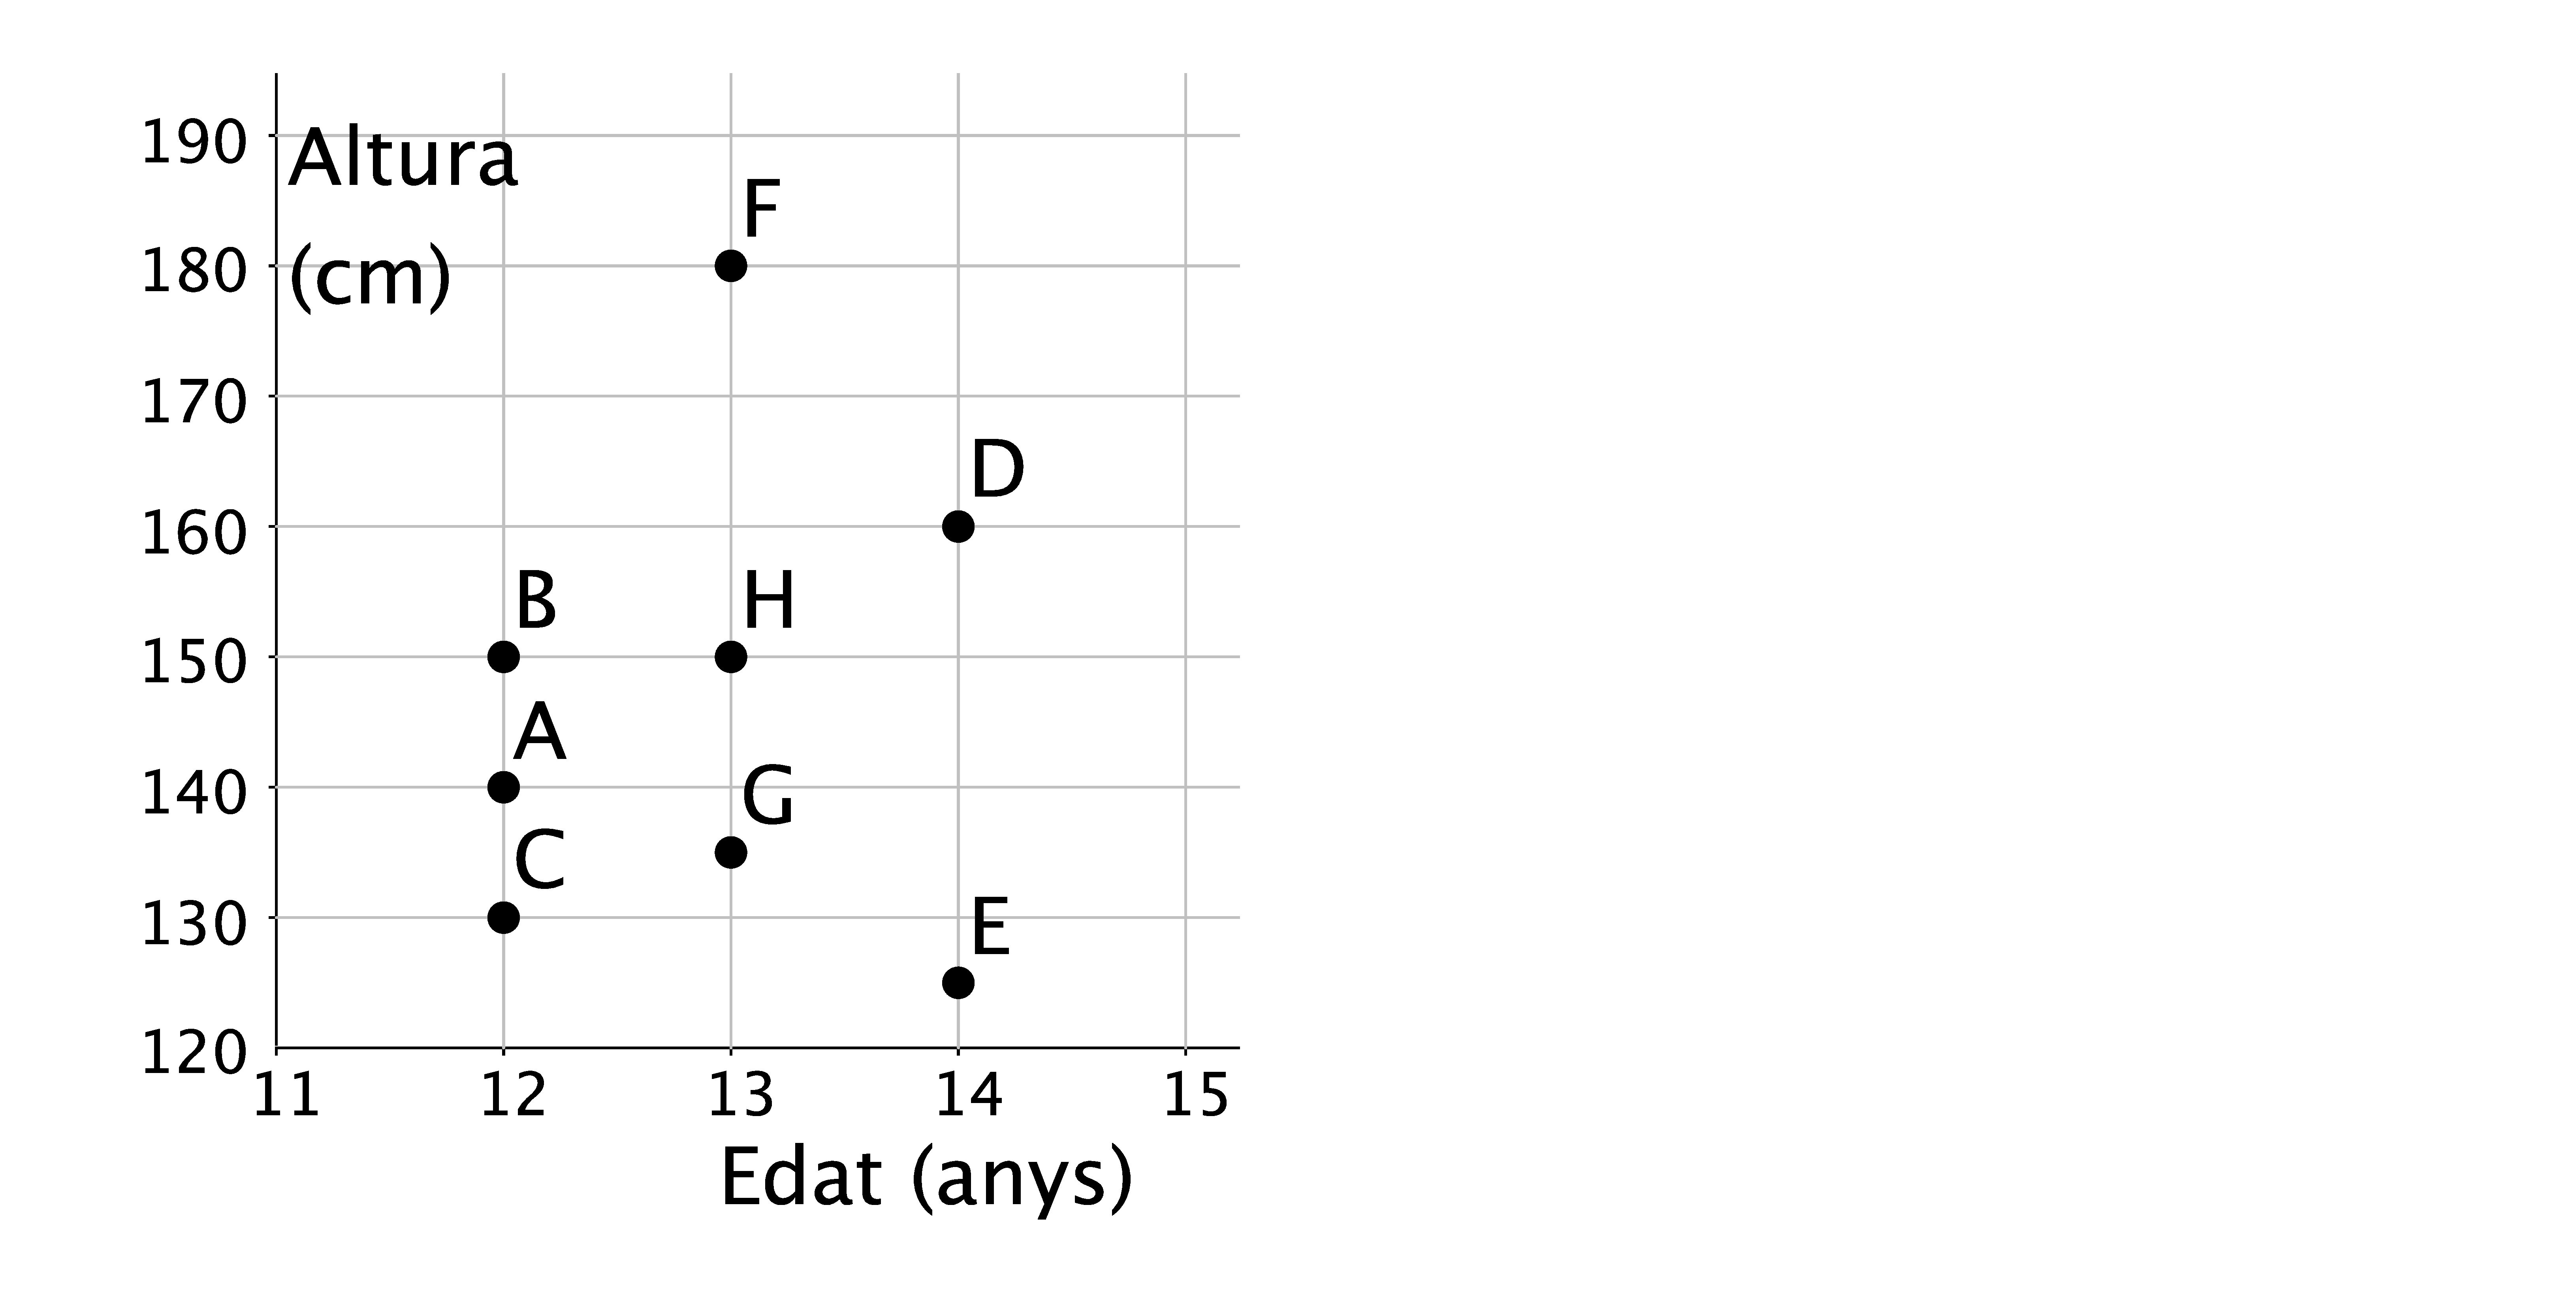
\includegraphics[width=4.5cm]{img-08/graf44}
\end{minipage}
\begin{minipage}{9cm}
	\begin{tasks}
		\task  Si en Joan té 14 anys, quina pot ser la seva altura? 
		\task  Si Maria mesura 180 cm, quina pot ser la seva edat? 
		\task  La relació entre l'altura i l'edat dels diferents components de l'equip, és una relació funcional? Per què?
		\task  I la relació entre l'edat i l'altura? Realitza una gràfica similar a l'anterior per representar aquesta situació.
	\end{tasks}
\end{minipage}
\end{mylist}

\answers[cols=1]{[125 o 160 cm, 13 anys, No és una relació funcional perquè per una edat trobam diverses altures, Tampoc és funcional perquè una una altura trobam diferents edats.]}

\section{La funció lineal i afí}
 

\begin{theorybox}
	

\video[rows=5,ytid=1BMng0\_9LK4]{191}{Funcions lineals i afins}
	
 Totes les gràfiques de les funcions $y=\text{''Polinomi de 1r grau''}$ són línies rectes.
 	
 Les funcions $y=mx$ són de \textbf{proporcionalitat directa o lineals}. \linebreak $m$ s'anomena el \textbf{pendent}.
 
 \begin{center}
 \begin{tabular}{lcl}
 	$m$ positiu & $\rightarrow$ & la recta és creixent \\
 	$m$ negatiu & $\rightarrow$  & la recta és decreixent \\
 	$m=0$ & $\rightarrow$  & la recta és constant o horitzontal.
 \end{tabular}
\end{center}

El pendent d'una recta s'obté de dividir el canvi de les $y$ entre el canvi de les $x$: $m=\frac{\Delta y}{\Delta x}$
 
\end{theorybox}

 


\subsection{Funcions lineals}

\begin{mylist}	
	
	\exer Representa aquestes funcions:
	\begin{tasks}(4)
		\task $y=2x$
		\task $y=\frac{3}{2}x$
		\task $y=-3x$
		\task $y=-\frac{4}{5}x$
	\end{tasks}
Indica en cada cas el seu pendent.
\answers{[$m=2$, $m=\frac{3}{2}$, $m=-3$, $m=\frac{-4}{5}$]}
	
	\exer  Escriu tres funcions que les seves gràfiques siguin tres rectes que passin per l'origen de coordenades i els seus pendents siguin 3, $-$2, i 1/2 respectivament.
\answers{$y=3x$; $y=-2x$; $y=\frac{1}{2}x$ }
	
	\exer Representa la recta que passa pels punts següents i calcula'n el seu pendent. Escriu l'equació de cada recta.
		\begin{tasks}(2)
		\task $A(0, 0)$ i $B(3, 1)$
		\task $A(-1, -2)$ i $B(2, 4)$
		\task $A(0, 0)$ i $B(-2, 5)$
		\task $A(-3, 4)$ i $B(3, -4)$
	\end{tasks}

\answers{[$m=\frac{1}{3}$; $y=\frac{1}{3}x$, $m=2$; $y=2x$, $m=-5/2$; $y=-\frac{5}{2}x$, $m=-4/3$; $y=-\frac{4}{3}x$]}
 
\exer  Un metre de certa tela costa 1,35 €, quant costen 5 metres? I 10 m? I 12,5 m? Quant costen ``\textit{x}'' metres de tela? Escriu la fórmula d'aquesta situació.
\answers{6.75 \euro{}, 13.5 \euro{}, 16.88 \euro{}. En general $y=1.35 x$}


\exer  Si el canvi d'euros a dollars està 1 € = 1,37\$, completa en el teu quadern la següent taula d'equivalència entre les dues monedes:

\begin{longtable}{|p{0.2in}|p{0.6in}|p{0.6in}|p{0.6in}|p{0.6in}|p{0.6in}|} \hline 
	\cellcolor{lightgray}\textbf{\euro{}} & 2 & 5 & 10 & 27 & 60 \\ [0.3cm] \hline 
	\cellcolor{lightgray}\textbf{\$} &  &  &  &  &  \\ [0.3cm] \hline 
\end{longtable}
Expressa mitjançant una fórmula la relació que existeix entre ambdues monedes. Es pot expressar de forma única aquesta relació? És una funció? Si realitzes el canvi en una oficina, et cobren una petita comissió fixa per realitzar l'operació d'1,5 €. Com quedarien les fórmules en aquest cas?

\answers{
	\begin{tabular}{|c|c|c|c|c|c|} \hline 
		\cellcolor{lightgray}\textbf{\euro{}} & 2 & 5 & 10 & 27 & 60 \\ [0.3cm] \hline 
		\cellcolor{lightgray}\textbf{\$} &2.74  & 6.85 & 13.70 & 36.99 &  82.20 \\ [0.3cm] \hline 
\end{tabular}\par
En general: $y=1.37 x$. És una funció.\par
Si aplicam comissió: $y=1.37 (x - 1.5)=1.37 x -2.06$; igual que abans però et lleven \$ 2.06
}

\exer  Un fabricant vol construir tassons cilíndrics mesuradors de volums, que tinguin de radi de la base 4 cm i d'altura total del tassó 24 cm. Escriu una fórmula que indiqui com varia el volum en anar variant l'altura del líquid. Construeix una taula amb els volums corresponents a les altures preses de 3 en 3 cm. Escriu també una fórmula que permeti obtenir l'altura coneixent els volums. A quina altura caldrà col·locar la marca per tenir un decilitre?

\answers{\begin{tabular}{|c|c|c|c|c|c|} \hline 
		\cellcolor{lightgray}\textbf{h} & 0 & 3 & 6 & 9 & 12 \\ [0.3cm] \hline 
		\cellcolor{lightgray}\textbf{V} & 0 & 151 & 301.4 & 452  & 603  \\ [0.3cm] \hline 
	\end{tabular}\par
$V=\pi r^2 h = 50.24 h$. $h=\frac{V}{50.24}$. 1 dl = 100 cm$^3$, aleshores aproximadament s'ha de col·locar la marca a 2 cm d'altura.
}

\exer  La distància, \textit{d}, recorreguda per un tren depèn del nombre de voltes, \textit{n}, que dóna cada roda de la locomotora. 
\begin{tasks}(1)
	\task Escriu la fórmula que permet obtenir \textit{d} conegut \textit{n}, sabent que el diàmetre de les rodes de la locomotora és de 78 cm.
	\task  Dibuixa la gràfica.
	\task Quina distància haurà recorregut el tren quan la roda hagi donat mil voltes? (pren com a valor de $\piup$ el número 3,14).
	\task Quantes voltes haurà donat la roda al cap de 7 km?
\end{tasks}

\answers[cols=1]{[$d=78\pi n$, Solució gràfica: una recta que passa per l'origen i té pendent $78\pi=245.04$, $d=78\pi\,1000=245\,044$ cm =2.45 km, 2856.6 voltes]}

\end{mylist}	
		
\subsection{Funcions afins}	

\begin{theorybox}
	 Les funcions del tipus $y=mx+n$ són línies rectes. $m$ s'anomena \textbf{pendent} i $n$ l'\textbf{ordenada a l'origen}. L'ordenada a l'origen és el punt on la recta talla l'eix de les Y.
	
	Les funcions $y=n$ són rectes horitzontals i s'anomenen funcions \textbf{constants}.  El seu pendent és igual a 0.
	
\end{theorybox}

\begin{mylist}		
	\exer  Fes una taula de valors i representa gràficament en el teu quadern: 
	\begin{tasks}(4)
		\task \textbf{$y=3x+2$}
		\task \textbf{$y=x-3$}
		\task \textbf{$y=-2x-1$}
		\task \textbf{$y=-\frac{x}{2}+4$}
	\end{tasks}
Indica en cada cas què val el pendent i l'ordenada a l'origen de cada recta.

\answers[cols=1]{[Pendent 3; ordenada 2, Pendent 1; ordenada --3, Pendent --2; ordenada --1, Pendent $-\frac{1}{2}$; ordenada 4]}

	\exer \mental Com són entre sí dues rectes d'igual pendent i diferent ordenada en l'origen?
	
	\answers{Són rectes paral·leles.}
	
	\exer  Dibuixa en els mateixos eixos de coordenades les rectes que passen pels següents punts:
	
	\begin{center}
	$A(0,0)$ i $B(1,-2)$  \quad \quad\quad \quad   $A(1,1)$ i $B(0,3)$    \quad \quad\quad \quad  $A(-2,0)$ i $B(0,-4)$
	\end{center}
	
	\begin{tasks}
		\task  Com són les rectes? 
		\task  Calcula l'equació de les tres rectes de l'apartat anterior. Què tenen en comú les equacions de les rectes?
	\end{tasks}

\answers[cols=1]{[Totes les rectes són paral·leles (i decreixents), $y=-2x$; $y=-2x+3$; $y=-2x-4$. Totes elles comparteixen el mateix pendent ($m=-2$) ]}


		
	\exer Troba l'equació i dibuixa la gràfica de les rectes següents:
	\begin{tasks}(1)
		\task   El seu pendent és 2 i la seva ordenada en l'origen és 3.
		\task   Passa pels punts \textit{A}( 1, 3) i \textit{B}(0, 4).
		\task   La seva ordenada en l'origen és 0 i el seu pendent és 0.
		\task   Passa pels punts \textit{C}($-$1, 3) i \textit{D}($-$2, 5).
	\end{tasks}
	

\answers{[$y=2x+3$, $y=-x+4$, $y=0$, $y=-2x+1$]}	
	
	\exer  Dibuixa en el teu quadern i calcula l'equació de les rectes següents:
	\begin{tasks}
		\task   De pendent 3 i ordenada en l'origen 0.
		\task   Passa pels punts $A( 2, 3)$ i $B(4, 1)$.
		\task   El seu pendent és 2 i Passa  pel punt (4, 5).
	\end{tasks}
	
\answers{[$y=3x$, $y=-x+5$, $y=2x-3$]}
	
	
\exer  Realitza en el teu quadern una taula de valors de la funció $e(\textit{t}) = 5\textit{t} + 20$, representa'ls gràficament i indica la figura que determinen. Si aquesta funció representa l'espai (en quilòmetres) que recorre una persona que duu caminats 20 km i camina a una velocitat de 5 km/h, en funció del temps que triga a recórrer-ho (en hores), indica quins serien els valors que no tindria sentit donar a la variable independent i en què es tradueix això en la gràfica. 
 
 
 \answers{\begin{tabular}[]{|c|c|c|c|c|c|c|}\hline
 		$t$ & 0 & 1 & 2 & 3 & 4 & 5 \\ \hline
 		$e$ & 20 & 25 & 30 & 35 & 40 & 45 \\ \hline
 \end{tabular} \par 
És una recta que passa per (0,20) i té pendent 5. No té sentit per temps negatius.
}
 
 \vspace{-4.5cm}
 \exer \begin{minipage}[t]{0.82\textwidth}
 	Un globus sonda utilitzat pel Servei Meteorològic dels Pirineus per mesurar la temperatura a diferents altures duu incorporat un termòmetre. S'observa que cada 180 m d'altura la temperatura disminueix un grau. Cert dia la temperatura en la superfície és de 9º C. Determina:\vspace{0.2cm}
 	
 	\begin{tasks}(1)
 		\task Quina temperatura hi haurà a 3 km d'altura? \vspace{0.1cm}
 		\task  A quina altura hi haurà una temperatura de $-$30º C? \vspace{0.1cm}
 		\task  Escriu una fórmula que permeti calcular la temperatura \textit{T} coneixent l'altura \textit{A}. Confecciona una taula i dibuixa la gràfica. Quin tipus de funció és? \vspace{0.1cm}
 		\task  Si la temperatura en la superfície és de 12º C, quina és llavors la fórmula? Quin tipus de funció és?
 	\end{tasks}
 \end{minipage}
 \hspace{0.5cm}
 \begin{minipage}{0.1\textwidth}
 	\centering
 	\vspace{4.5cm}
 	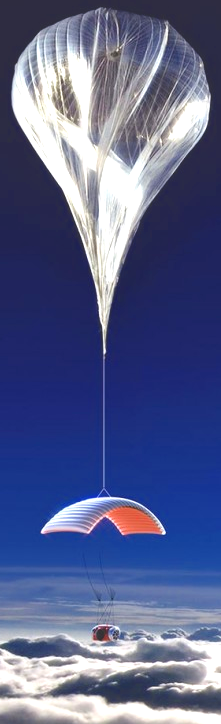
\includegraphics[width=\textwidth]{img-08/globo-sonda}
 \end{minipage}
 
 \answers[cols=1]{[--7.6 $^\circ$C, 7020 m, $t=9-\frac{a}{180}$, $t=12-\frac{a}{180}$. Les dues funcions afins representen rectes paral·les.]}

 \exer  Una empresa de lloguer de vehicles ofereix dues fórmules diferents. 
 
 \textit{Fórmula 1:} Lloga per 300 euros al dia amb quilometratge il·limitat. 
 
 \textit{Fórmula 2:} Lloga per 200 euros al dia i 7 euros el quilòmetre. 
 
 Volem fer un viatge de 10 dies i mil quilòmetres, quant ens costarà amb cadascuna de les fórmules? Com no sabem el quilometratge exacte que acabarem fent, ens interessa fer un estudi per saber la fórmula més beneficiosa. Escriu les fórmules d'ambdues situacions i dibuixes les seves gràfiques. Raona, a partir d'aquestes gràfiques, quina fórmula és més rendible segons el nombre de quilòmetres que anem a fer.
 
 \answers{Fórmula 1: $y=3000d$. Fórmula 2: $y=200d + 7x$. El cost de la fórmula 1: 3000 \euro{}. El cost de la fórmula 2: 2000+7000=9000 \euro{}. En general és més econòmica l'opció 1; però si hem de fer menys de 14 km diaris surt més econòmica la fórmula 2.}
 
 
\exer \ggb  Calcula dos punts de les rectes d'equacions: $y=2x+2$ i $y=-\frac{x}{2} +2$, per dibuixar-les amb Geogebra. Indica dues propietats comunes d'ambdues gràfiques. 

Representa, també, les rectes d'equacions: $y=-3x+1$ i $y=\frac{x}{3} -3$. 

Quina condició compleixen els pendents de dues rectes perpendiculars?

\answers{Les parelles de rectes són perpendiculars. La condició que han de complir és $m \cdot m' = -1$}
 
\exer  Escriu l'equació de la recta paral·lela a  $y=4x + 2$  d'ordenada en l'origen 6.

\answers{$y=4x+6$}

\exer  Sense representar-los gràficament, digues si estan alineats els punts \textit{A}( 3, 4), \textit{B}(7, 9) i \textit{C}(13, 15). \textit{Ajuda: } Els pendents $m_{AB}$ i $m_{BC}$ han d'ésser iguals.

\answers{No estan alineats. Els punts A,B estan sobre una recta de pendent 5/4, mentre que els punts B,C estan sobre una recta de  1.}

\end{mylist}




\section{La funció quadràtica o paràbola}

\begin{theorybox}
	\video[ytid=03sdgaI3drg]{192}{Funcions quadràtiques o paràboles}


Tots els polinomis de segon grau com $y=ax^2+bx+c$ són \textbf{funcions quadràtiques o paràboles}. Possiblement et recordi de la forma que té una antena parabòlica.


$a$ controla l'obertura i la forma de la paràbola. 
\begin{itemize}
	\item Si $a$ és positiu la paràbola és \textbf{còncava} $\cup$. Té un mínim.
	\item Si $a$ és negatiu la paràbola és \textbf{còncava} $\cap$. Té un màxim.
\end{itemize}

El \textbf{màxim o mínim} de la paràbola s'anomena el \textbf{vèrtex}.

En canvi, els nombres $b$ i $c$ controlen la \textbf{posició del vèrtex}, que podem obtenir de la fórmula:

\begin{minipage}{0.7\textwidth}
\begin{equation*}
x_v = \frac{-b}{2a}
\end{equation*}
La $y_v$ s'obté substituint la $x_v$ dins de l'equació de la paràbola.

Les paràboles compleixen que són \textbf{simètriques} respecte del vèrtex.
\end{minipage}
\begin{minipage}{0.25\textwidth}
	\centering
	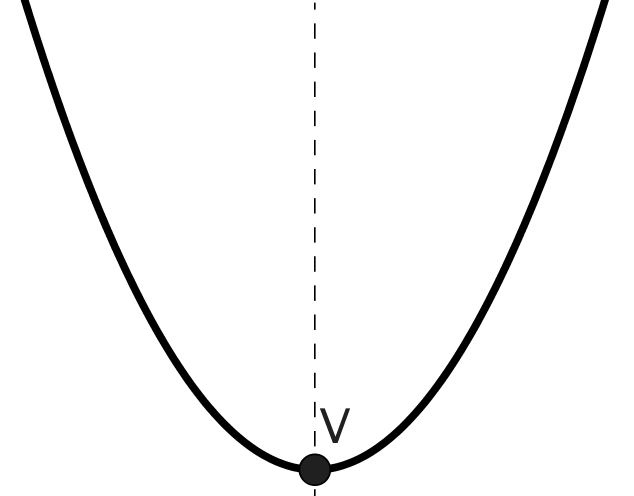
\includegraphics[width=0.9\textwidth]{img-08/parabola}
\end{minipage}
\end{theorybox}	


\begin{mylist}


\exer  Dibuixa en el teu quadern les gràfiques de les paràboles: 
\begin{tasks}(2)
	\task  $y =  \textit{x}^{2}$   
	\task  $y = 2 \textit{x}^{2}$
	%\task  $y = 1/3\textit{x}^{2}$
	\task  $y =\textit{$-$x}^{2}$
	%\task  $y = $-$1/2\textit{x}^{2}$;
	\task  $y = -3\textit{x}^{2}$. 
\end{tasks}
Indica si són còncaves o convexes. Comprova que totes elles passen per l'origen.

\answers{a), b) còncaves. c), d) convexes.\par 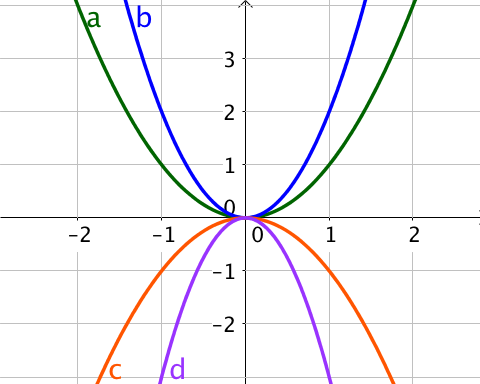
\includegraphics[width=0.45\textwidth]{img-sol/t8-29}}

\exer  Fes una taula de valors i representa gràficament en el teu quadern: 
\begin{tasks}(3)
\task { $y=1 - x^2$}
\task  {$y=2x^{2} -8$}
\task {$y=-3x^{2} +6x-4$}
\end{tasks}
 \answers{Gràfics:\par 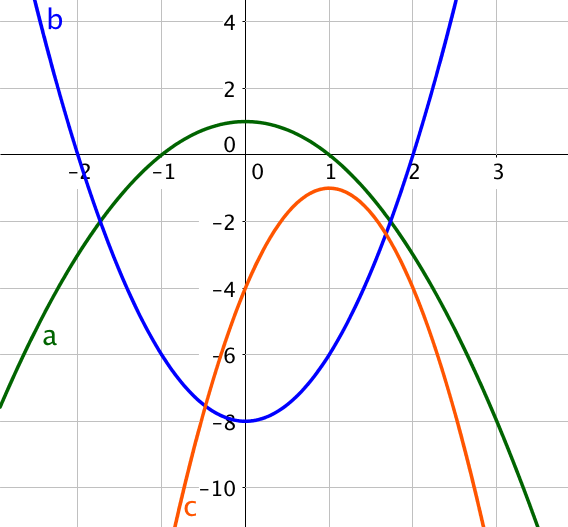
\includegraphics[width=0.38\textwidth]{img-sol/t8-30}}
 
 \exer  Determina el vèrtex de les següents paràboles i dibuixa la seva gràfica:
 
 \begin{tasks}(2)
 	\task  \textit{y =} 2\textit{x}${}^{2}$ + 8\textit{x} + 12                       
 	\task  \textit{y =} --2\textit{x}${}^{2}$ + 8\textit{x} -- 10            
 	\task  \textit{y =} 2\textit{x}${}^{2}$ -- 4\textit{x} + 2  
 	\task  \textit{y =} 2\textit{x}${}^{2}$ + 6\textit{x}
 \end{tasks}

\answers{[$V(-2,4)$, $V(2,-2)$, $V(1,0)$, $V(-\frac{3}{2},-\frac{9}{2})$]}

\end{mylist}
  \vspace{-0.4cm}
 \begin{example}
 	
 	a)  \textit{y =} 2\textit{x}${}^{2}$ + 8\textit{x} +2. Aquesta paràbola té $a=2$ i $b=8$.  L'abscissa del vèrtex s'obté de \linebreak $x_v =\frac{-8}{2\cdot 2}=-2$. La $y_v = 2 \cdot (-2)^2 + 8\cdot(-2) + 2  = -6$. El vèrtex es troba en el punt $V(-2, -6)$. 
 	
 	Per representar la paràbola feim una taula de valors al voltant del vèrtex:
 	
 	\begin{minipage}{0.4\textwidth}
 		\centering
 		\begin{tabular}{l|l}
 			x & y \\
 			\hline 
 			-4 & 2\\
 			-3 & -4\\
 			-2 & -6\\
 			-1 & -4\\
 			0 & 2\\
 		\end{tabular}
 	\end{minipage}
 	\begin{minipage}{0.4\textwidth}
 		\centering
 		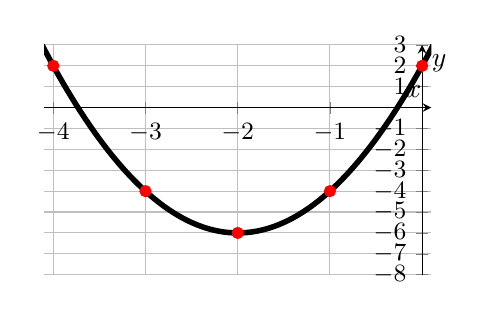
\begin{tikzpicture}[]
 		\begin{axis}[width=6.5cm,height=4.5cm, axis background/.style={fill=white}, axis lines=middle, 
 		grid = major,
 		xlabel=$\small x$,
 		ylabel=$\small y$, 
 		xtick={-5,-4,...,3},
 		ytick={-8,-7,...,3},
 		ymin = -8,
 		ymax = 3,
 		tick label style={font=\small},
 		legend style={font=\small,legend pos=outer north east},]
 		\addplot[ samples=201, line width=2pt]{2*x^2+8*x+2};
 		\addplot[red, mark=*, only marks] coordinates{(-4,2) (-3,-4) (-2,-6) (-1,-4) (0,2) };	
 		\end{axis}
 		\end{tikzpicture}
 	\end{minipage}
 \end{example}

\begin{mylist}
	

\exer  Calcula el vèrtex, l'eix de simetria i els punts d'intersecció amb els eixos de les següents paràboles. Dibuixa les seves gràfiques.

\begin{tasks}(2)
	\task  \textit{y =} \textit{x}${}^{2}$ + 8\textit{x} -- 13                          
	\task  \textit{y =} --\textit{x}${}^{2}$ + 8\textit{x} -- 13          
	\task  \textit{y =} \textit{x}${}^{2}$ -- 4\textit{x} + 2  
	\task  \textit{y =} \textit{x}${}^{2}$ + 6\textit{x                                  }
%	\task  \textit{y =} --\textit{x}${}^{2}$ + 4\textit{x} -- 7 \textit{}
\end{tasks}


\answers[cols=1]{[$V(-4,-29)$; talls $(-9.39,0)$ $(1.39,0)$ $(0,-13)$,
		  $V(4,3)$; talls $(2.27,0)$ $(5.73,0)$ $(0,-13)$,
		  $V(2,-2)$; talls $(0.59,0)$ $(3.41,0)$ $(0,2)$,
		  $V(-3,-9)$; talls $(-6,0)$ $(0,0)$ ]}


\exer \spen Completa aquest resum. En la gràfica de $y = ax^{2}$:
\begin{tasks} 
\task Si  $a > 0$ llavors té curvatura \quad \textsc{còncava} / \textsc{convexa}.
%
\task  Si $a > 1$ llavors té una obertura \quad \textsc{menor} / \textsc{major} \quad que $y=x^{2}$.
%
\task Si  $a < 0$ llavors té curvatura \quad \textsc{còncava} / \textsc{convexa}.
%
\task Si $-1<a<0$ llavors té una obertura \quad \textsc{menor} / \textsc{major} \quad que $y=x^{2}$.
\end{tasks}

\answers{[còncava, menor, convexa, major]}

	\vspace{-2.5cm}
\exer  \begin{minipage}[t]{0.65\textwidth}
	El pont \textit{Golden Gate} permet la comunicació entre els dos costats de la badia de San Francisco. Les seves torres, de 746~peus d'altura, estan separades per una distància d'uns 4200 peus. La calçada, que té una amplada de 90 peus i es troba a una altura de 220 peus sobre el nivell de l'aigua, està subjecta a les torres mitjançant dos cables, de 3 peus de diàmetre, que tenen forma de \textbf{paràbola} i que toquen la calçada en el centre del pont. 
\end{minipage}
\begin{minipage}{0.25\textwidth}
	\vspace{2.5cm}
	\raggedright
	\includegraphics*[width=1.1\textwidth]{img-08/goldenbridge}
\end{minipage}

\begin{tasks} 
%	\task  Realitza un dibuix on quedin reflectits les dades més significatives del problema.
	\task  Determina la relació que existeix entre l'altura a la qual es troba un punt del cable i la distància de la seva projecció vertical al  centre del pont. 
	\task  Aplica aquesta fórmula per calcular l'altura d'un punt del cable que la seva vertical està a 1000 peus del centre del pont.
\end{tasks}

\answers{[Respecte el centre el pont $y=0.0001193 x^2$, 119.27 peus d'altura]}

\end{mylist}
 

\begin{mylist}
	
	\exer  Escriu l'equació d'una paràbola d'igual forma que \textit{y =} \textit{x}${}^{2}$, però traslladada 5 unitats en sentit horitzontal a la dreta i 3 unitats en sentit vertical cap amunt. Quines coordenades té el seu vèrtex?
	
	\answers{$y=(x-5)^2+3 = x^2-10x+28$. El nou vèrtex és $V(5,3)$.}
	
	\exer  Un rectangle té un perímetre de 100 cm. Si anomenam \textit{x} a la longitud d'un dels seus costats, escriu la fórmula que dóna l'àrea en funció de \textit{x} . Dibuixa la seva gràfica. Quin tipus de funció és?
	
	\answers{$A=-x^2+50x$. És una funció quadràtica que talla a l'eix de les abscisses a $x=0$ i $x=50$ i vèrtex $V(25, 625)$ } 
	
	\exer  Una caixa quadrada té una altura de 20 cm. Com depèn el seu volum del costat de la base? Dibuixa la gràfica de la funció que resulta.
	
	\answers{$V=20x^2$}
	
	\exer  Amb un full de paper de 32 cm de llarg i 22 cm d'ample es retalla un quadrat de 2 cm de costat en cadascuna de les cantonades, es doblega i es construeix una caixa. Quin és el volum de la caixa? I si es retallen quadrats de 3 cm? Quin és el volum si el costat del quadrat retallat és\textit{ x}? Escriu la fórmula i dibuixa la gràfica.

\answers{$V = (32 – 2x) \cdot (22 – 2x)\cdot x$; $V(3) = 1248$ cm$^3$; $V(2) = 1 008$ cm$^3$}





\end{mylist}
 


\section{Interpretació i característiques de les funcions}


\begin{mylist}
	
	\exer  Assenyala totes les característiques que puguis de les funcions representades mitjançant les seves gràfiques: domini i recorregut, simetria, punts d'intersecció amb els eixos de coordenades, continuïtat, creixement i decreixement, màxims i mínims, periodicitat.
\begin{center}
\begin{tabular}{|c|c|} \hline 
 \rowcolor{lightgray}	GRÀFICA 1 & GRÀFICA 2 \\ \hline
	{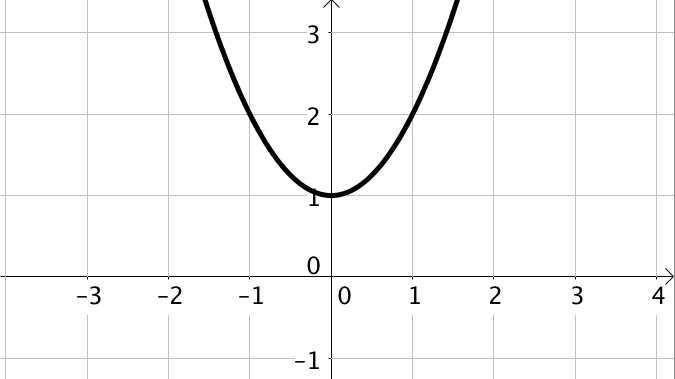
\includegraphics[width=0.35\textwidth]{img-08/graf1}} & {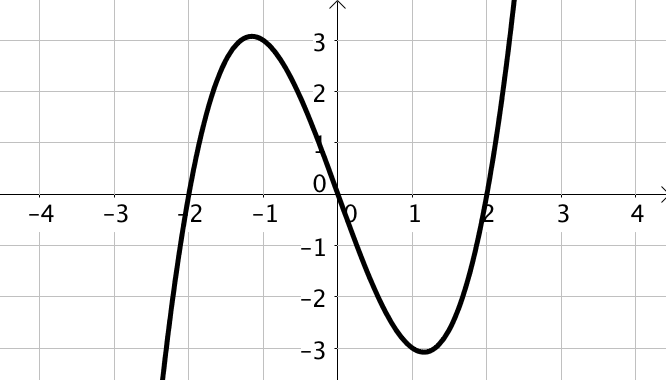
\includegraphics[width=0.35\textwidth]{img-08/graf2}} \\ \hline
	\rowcolor{lightgray} GRÀFICA 3 & GRÀFICA 4 \\ \hline 
	 {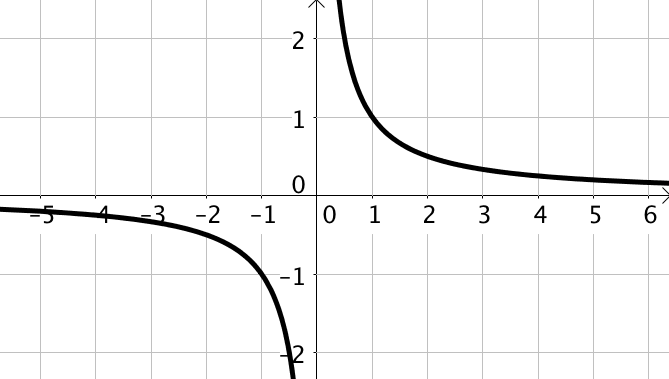
\includegraphics[width=0.35\textwidth]{img-08/graf3}} & {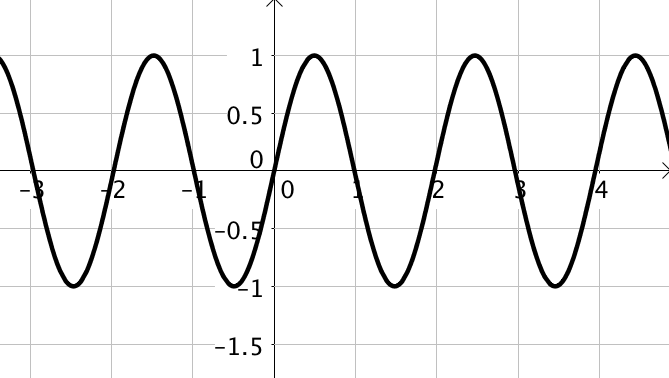
\includegraphics[width=0.35\textwidth]{img-08/graf4}} \\ \hline 
\end{tabular}
\end{center}

\answers[cols=1]{[Gràfica 1: Dom $f=\Re$; Rec $f=[1,+\infty]$; Simetria parell; Talla eix OY a (0,1); És contínua; És decreixent $(-\infy,0)$ i creixent de $(0,+\infty)$; Té un mínim a (0,1),
		Gràfica 2: Dom $f=\Re$; Rec $f=\Re$; Simetria senar; Talla eix OX (--2,0) (0,0) (2,0) i l'eix OY a (0,0); És contínua; És decreixent $(-1,1)$ i creixent de $(-\infty,-1)\cup(1,+\infty)$; Té un màxim a (-1,3) i un mínim a (1,-3),
		Gràfica 3: Dom $f=\Re$-{0}; Rec $f=\Re-{0}$; Simetria senar; No hi ha talls amb eixos; No és contínua a x=0; Sempre decreixent; No té extrems,
		Gràfica 4: Dom $f=\Re$; Rec $f=[-1,1]$; Simetria senar; Talla l'eix OX a cada nombre enter; És contínua; És periòdica amb període 2. Presenta màxims a $0.5+2n$ i mínims $1.5+2n$ 
		]}


\exer  Joaquim ha arribat a un acord amb el seu pare per rebre la seva paga. Cobrarà 20~€ al mes el primer any, i 5~€ més per cada any que passi. Quant li correspondrà dins de 7 anys? Fes una taula de valors i representa la seva gràfica. És contínua? Indica els punts de discontinuïtat i el seu tipus. Busca una fórmula que permeti calcular la paga quan hagin passat \textit{n} anys.

\answers{
	D'aquí a 7 anys cobrarà 50 euros. És una funció esglaonada, ja que cobra el mateix durant tot un any, i després augmenta 5 euros:\par  $P =\left\{ \begin{array}{cl} 20 & \text{1r any} \\
	25 & \text{2n any} \\ 30 & \text{3r any} \\ \cdots & \\ 20 + 5(n-1) & \text{any }n  \end{array} \right.$}

	\exer  
	El consum de gasolina i gasoil d'un cotxe per cada 100 km ve representat mitjançant la gràfica.
	
	\begin{minipage}{0.4\textwidth}
		\centering
		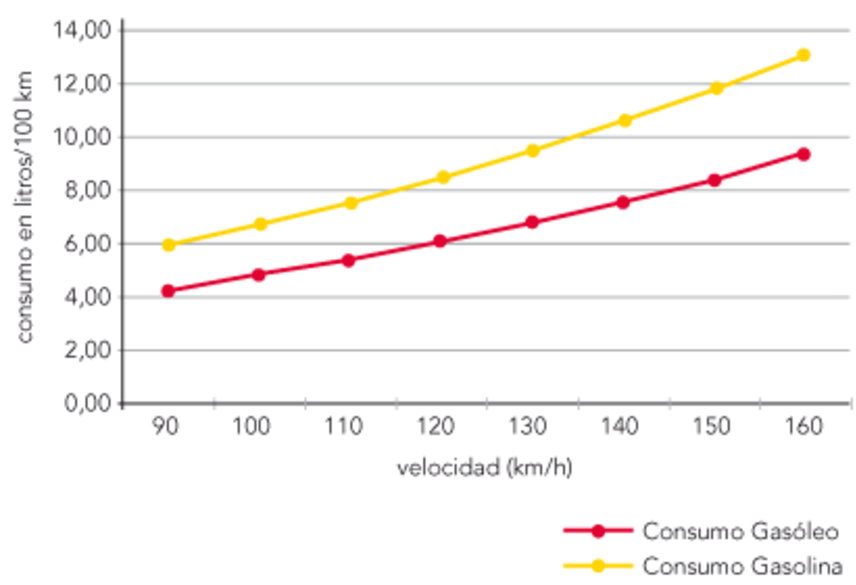
\includegraphics[height=4.5cm]{img-08/consumo}
	\end{minipage}
	\begin{minipage}{0.55\textwidth}
	\begin{tasks}(1)
		\task  Quina és la variable depenent? 
		\task  I la independent?
		\task  Quin és el consum per a una velocitat de 160 km/h?
		\task  A quina velocitat el consum és de 7 l/100 km?
		\task  Utilitza la gràfica per explicar com vària el consum de combustible depenent de la velocitat del cotxe.
	\end{tasks}
	\end{minipage}

\answers[cols=1]{[El consum en litres/100 km, La velocitat en km/h, Gasoil: 9.50 l/100 km; Benzina: 13 l/100 km, Gasoil: 135 km/h; Benzina: 105 km/h, El consum en general augment amb la velocitat i sempre és major el consum de benzina que no pas el de Gasoil.]}
  
 \exer La següent gràfica resumeix l'excursió que hem realitzat per la serra de Tramuntana:
		
	\begin{minipage}{0.4\textwidth}
		\centering
		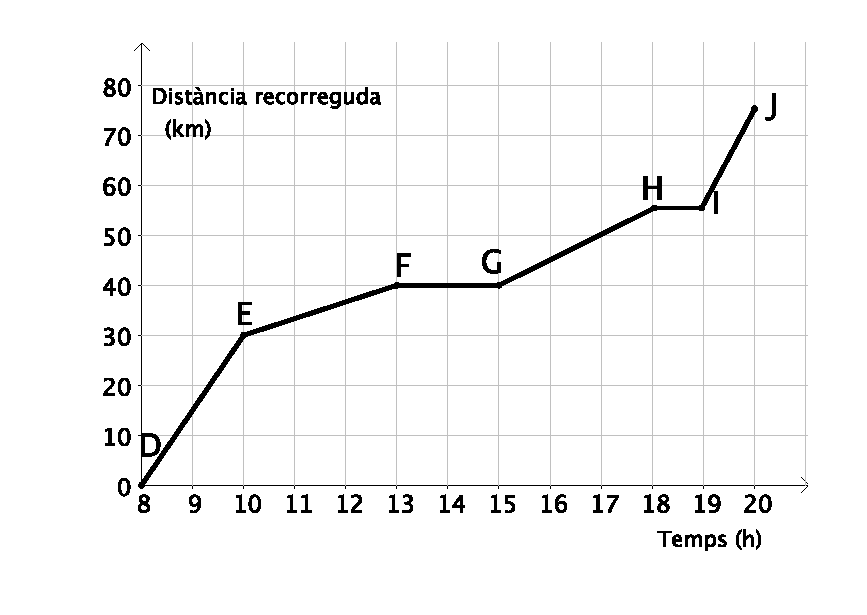
\includegraphics[width=6.2cm]{img-08/graf45}
	\end{minipage}
	\begin{minipage}{0.53\textwidth}
	\begin{tasks}
		\task Quant temps va durar l'excursió?
		\task  Quant temps es va descansar? A quines hores?
		\task  Quants quilòmetres es van recórrer?
		\task  En quins intervals de temps es va anar més ràpid que entre les 11 i les 13 hores?
		\task  Fes una breu descripció del desenvolupament de l'excursió.
		%\task  Construeix una taula de valors a partir dels punts assenyalats en la gràfica.
		%\task  Si en l'eix d'ordenades representéssim la variable ``distància al punt de partida'', seria la mateixa gràfica? Amb les dades que disposes, pots fer-la?
	\end{tasks}
	
\end{minipage}

\answers[cols=1]{[12 hores, 3 hores de descans: entre les 14 i les 15 i entre les 18 i les 19 hores, Es van recórrer 80 km, En tots els altres excepte quan descansaven, lliure]} 

\exer  Durant un viatge, la velocitat del cotxe varia depenent del tipus de carretera, de les condicions en què es troba, del temps meteorològic{\dots} La següent gràfica reflecteix la velocitat d'un vehicle en cada instant del trajecte que ha seguit.
 
 
	\begin{minipage}{0.5\textwidth}
	\begin{tasks}
	\task  És funcional la relació de dependència entre el temps i la velocitat?
	\task  Quina és la variable independent? I la depenent?
	\task  A quina velocitat anava quan duia una hora de viatge? En quins moments anava a una velocitat de 40 km/h?
		\task  Indica els intervals en els quals la velocitat ha augmentat i disminuït. Ha estat constant en algun moment? Quan? Durant quant de temps?
	\end{tasks}
	\end{minipage}
	\begin{minipage}{0.5\textwidth}
		\centering
		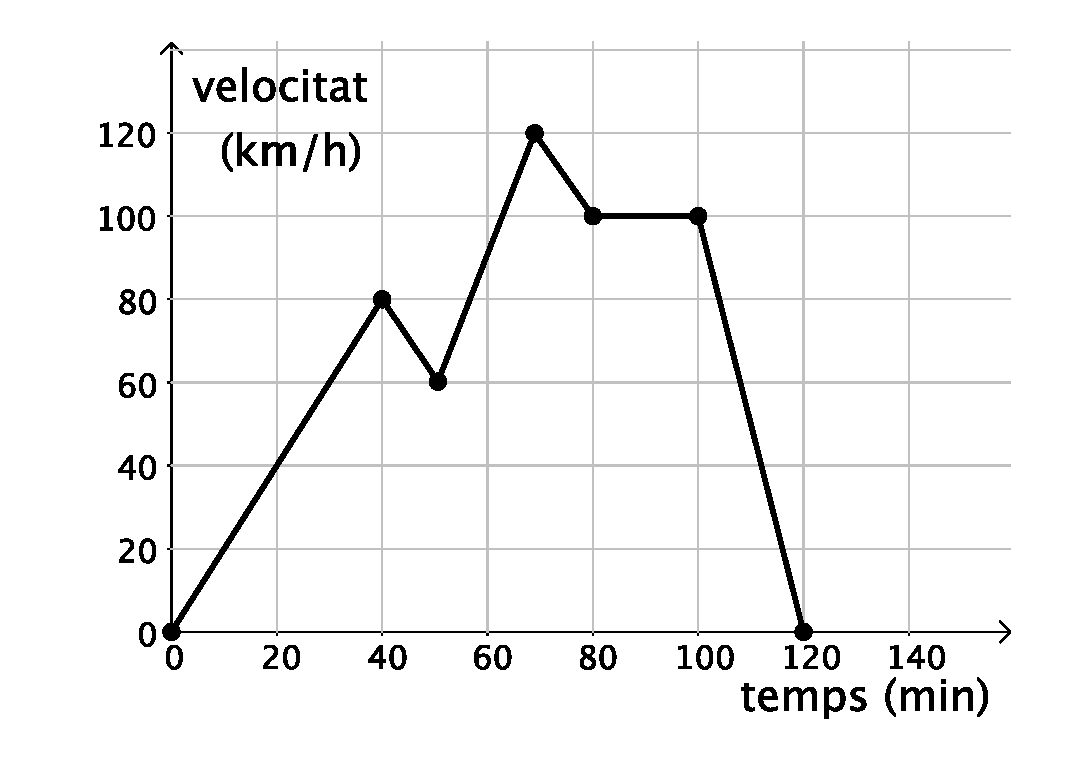
\includegraphics[width=6.5cm]{img-08/graf43.pdf}
	\end{minipage}
\begin{tasks}
	\task[e)]  Quins són els màxims i mínims relatius de la funció? 
\end{tasks}

 
 \answers[cols=1]{[Sí. Es funcional, Independent: temps; Dependent: Velocitat, Anava a 90 km/h; Anava a 40 km/h als 20 i 110 minuts, Creixent $(0,40)\cup (50,70)$; Decreixent $(40,50)\cup (70,80)\cup (100,120)$; Constant: $(80,100)$ durant 20 minuts, 
 	Els màxims relatius són (40,80) i (70,120); El mínim relatiu és (50,60). ]} 
 
\vspace{-1.75cm}
\exer \begin{minipage}[t]{0.7\textwidth}
	 Una ciutat té implantada l'ordenança de regulació de l'aparcament (ORA). La norma indica que s'ha de pagar una certa quantitat per cada minut d'aparcament i que hi ha d'haver un mínim de preu. En Joan posa 1,35 \euro{} i el parquímetre indica que disposa de 45 minuts. Sara amb 0,84 \euro{} només té 28 minuts.

\end{minipage}
\begin{minipage}{0.3\textwidth}
	\centering
	\vspace{1.5cm}
	
\includegraphics[width=0.5\textwidth]{img-08/ora}
\end{minipage}
	\begin{tasks}(1)
	\task Troba l'equació de la funció lineal $y=mx+n$ que relaciona el temps $x$ amb el preu $y$.
	\task Quant hem de pagar per un aparcament de 55 minuts?	
	\task Si hem pagam 2,40 \euro{} de quant de temps disposam?
\end{tasks}
 
\answers[cols=1]{[$y=0.03 x$, $1.65$ \euro{}, 80 minuts]}
 

\exer  En estudiar el creixement d'una planta observem que durant els primers 30 dies ho fa molt de pressa, en els 15 dies següents el creixement és més lent i després es manté amb la mateixa altura. Realitza un esbós de la gràfica que relaciona el temps amb l'altura aconseguida per la planta.


 Si tenim més informació podem millorar l'esbós. Per exemple, fes la taula i la gràfica en el cas que el creixement de la planta s'ajusti a les següents fórmules (el temps s'expressa en dies i l'altura en centímetres):
\begin{tasks}(1)
\task  Durant els primers 30 dies:  altura = 4 $\cdot$ temps
\task En els dies 30 a 45: altura = 90 + temps
 \end{tasks}

\answers{Gràfica: \par 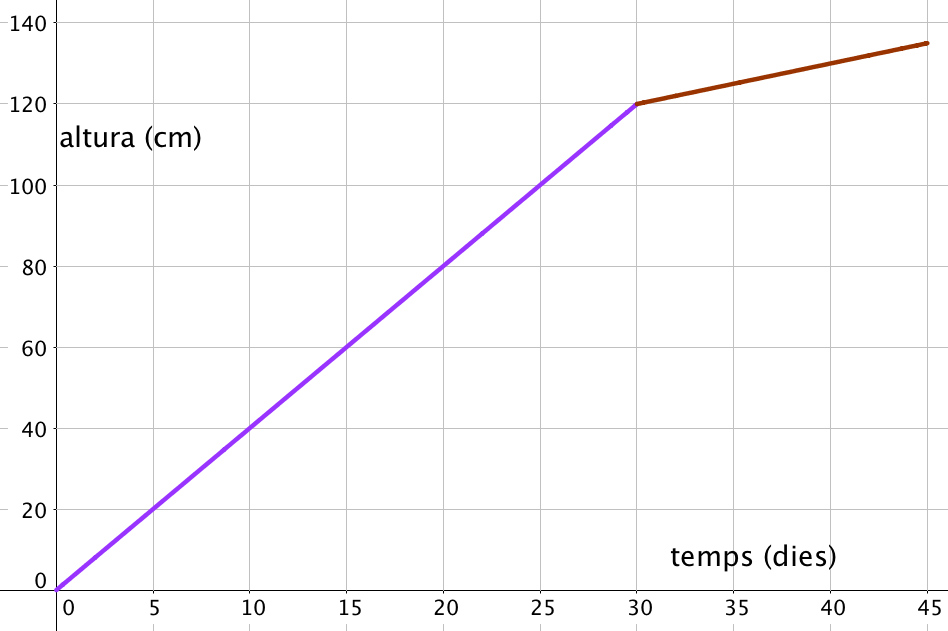
\includegraphics[width=0.45\textwidth]{img-sol/t8-45}}

\begin{comment}
\exer  Un viatge realitzat per un tren, en un cert interval de temps, ve donat de la següent forma:
\begin{itemize}
 \exer Durant les dues primeres hores, la distancia ``$d$'' (en quilòmetres) al punt de partida és $2t+1$, on ``$t$'' és el temps (en hores) de durada del trajecte.

 \exer Entre la 2a i 3a hora, aquesta distància ve donada per $-t+7$.

 \exer Entre la 3a i 4a hora, ambdues inclusivament, $d=4$.

 \exer Des de la 4a i fins a la 6a (inclusivament), la distància s'ajusta a $3t-8$.
\end{itemize}

Realitza una taula i una gràfica que reculli aquest viatge de la forma més precisa possible (per a això has de calcular, com a mínim, els valors de la variable temps en els instants 0, 2, 3, 4 i 6).
\begin{tasks}(1)
   \task Explica si la relació anteriorment explicada entre la distància recorreguda i el temps trigat a recórrer-la és funcional.
   \task La relació anterior, presenta alguna discontinuïtat?
   \task En quin moment la distància al punt de partida és de 7 km?
   \task Què indiquen els punts de tall de la gràfica amb els eixos?
   \task Determina els intervals on la funció és creixent, decreixent i constant.
   \task Troba els punts on la funció assoleix els seus màxims i mínims relatius i absoluts. Interpreta el significat que puguin tenir.
\end{tasks}



\exer  Representa gràficament les següents funcions, estudiant en ella totes les característiques que s'han treballat en el tema: monotonia, extrems, simetria i periodicitat.
\begin{tasks}(1)
  \task Valor absolut d'un nombre: $f\left(x\right)=\left|x\right|$.
   \task Oposat i invers d'un nombre: $f\left(x\right)=\frac{-1}{x} $.
   \task \textit{Mantissa} (a cada nombre li correspon la diferència entre aquest nombre i la seva part enter
  : $M\left(x\right)=x-E\left(x\right)$.
\end{tasks}


\exer  Les gràfiques següents mostren l'evolució, un dia qualsevol, de la temperatura aconseguida entre les 7 del matí i les 4 de la tarda en quatre ciutats (Madrid, Granada, Valladolid i Sevilla):


\begin{longtable}{|p{0.24\textwidth}|p{0.24\textwidth}|p{0.24\textwidth}|p{0.24\textwidth}|} \hline 
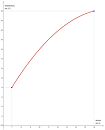
\includegraphics[width=0.2\textwidth]{img-08/image13.png} & \includegraphics*[width=0.2\textwidth]{img-08/image14.png} & \includegraphics*[width=0.2\textwidth]{img-08/image15.png} & \includegraphics*[width=0.2\textwidth]{img-08/image16.png} \\ \hline 
\end{longtable}

\begin{tasks}
\task  Estudia la monotonia de totes les gràfiques.
\task   En alguna ciutat la temperatura s'ha mantingut constant durant tot l'interval? I en part d'ell?
\task   Quina ciutat creus que presenta un canvi de temperatura més suau al llarg de tot el matí?
\task   Tenint en compte que a Madrid l'increment de la temperatura ha estat sempre lineal, a Granada la temperatura mínima s'ha aconseguit després de les 7 h i a Valladolid a partir del mig dia la temperatura va baixar, indica quina gràfica correspon a cadascuna de les ciutats i explica quins han estat les temperatures màximes i mínimes en cadascuna d'elles.
\end{tasks}
\end{comment}
\end{mylist}


\begin{autoaval}{38}
\begin{mylist}

 
\exer[2] L'únic punt que té ordenada negativa i es troba al 3r quadrant és:
\begin{tasks}(4)
\task $(-1,1)$
\task $(-1,-1)$
\task $(-1,0)$
\task $(1,-1)$
\end{tasks}  
\answers{\textbf{--6.} Autoavaluació: 1b; 2d; 3a; 4c; 5b; 6b}

\exer L'única taula que no correspon a una relació funcional és:
\begin{tasks}(4)
\task \begin{tabular}{|c|c|}
	\hline
	\rowcolor{lightgray} $x$ & $y$ \\
	\hline
 	0 & 1 \\ 
	\hline 
	1 & 2 \\ 
	\hline 
	2 & 3 \\ 
	\hline 
	3 & 4 \\ 
	\hline 
\end{tabular} 
\task  \begin{tabular}{|c|c|}
	\hline
	\rowcolor{lightgray} $x$ & $y$ \\
	\hline
	0 & 1 \\ 
	\hline 
	1 & 1 \\ 
	\hline 
	2 & 1 \\ 
	\hline 
	3 & 1 \\ 
	\hline 
\end{tabular} 
\task  \begin{tabular}{|c|c|}
	\hline
	\rowcolor{lightgray} $x$ & $y$ \\
	\hline
	0 & --1 \\ 
	\hline 
	1 & --1 \\ 
	\hline 
	2 & --2 \\ 
	\hline 
	3 & --3 \\ 
	\hline 
\end{tabular} 
\task  \begin{tabular}{|c|c|}
	\hline
	\rowcolor{lightgray} $x$ & $y$ \\
	\hline
	0 & 0 \\ 
	\hline 
	1 & 1 \\ 
	\hline 
	2 & 2 \\ 
	\hline 
	0 & --3 \\ 
	\hline 
\end{tabular}  
\end{tasks}

  
 
\exer  L'única funció afí que passa per l'origen de coordenades és 
\begin{tasks}(4)
\task $y = -4x$
\task $y = 3x + 1 $
\task $y = -2x + 3$
\task $y = -x - 1$
\end{tasks}

\exer L'única funció quadràtica és:
\begin{tasks}(4)
\task $y = -2x$
\task $y = 3x + 1 $
\task $y = -2x^2 + 3x$
\task $y = -x^3 - 1$
\end{tasks}
 

\exer La funció quadràtica que té el seu vèrtex en el punt (3, 9) és:
\begin{tasks}(4)
	\task $y = -2x^{2}$
	\task $y = -x^{2} +6x$
	\task $y = 3x^{2}-x + 1$
	\task $y = -2x^{2} + 3x$
\end{tasks}
 
\exer La única funció que és periòdica és:
\begin{tasks}(4)
	\task
	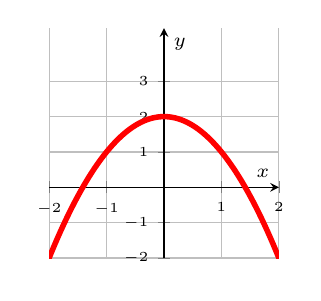
\begin{tikzpicture}[]
	\begin{axis}[width=4.5cm,height=4.5cm, axis background/.style={fill=white}, axis lines=middle, 
	grid = major,
	xlabel=$\scriptstyle x$,
	ylabel=$\scriptstyle y$, 
	xtick={-3,-2,...,5},
	ytick={-3,-2,...,3},
	ymin = -2,
	ymax = 4.5,
	tick label style={font=\tiny},
	legend style={font=\footnotesize,legend pos=outer north east},]
	\addplot[red, samples=201, line width=2pt]{-x^2+2};	
	\end{axis}
	\end{tikzpicture}
	\task 	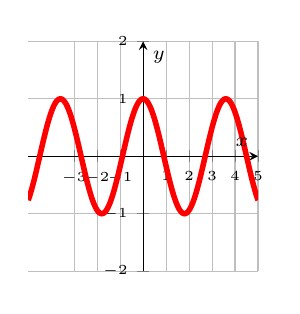
\begin{tikzpicture}[]
	\begin{axis}[width=4.5cm,height=4.5cm, axis background/.style={fill=white}, axis lines=middle, 
	grid = major,
	xlabel=$\scriptstyle x$,
	ylabel=$\scriptstyle y$, 
	xtick={-3,-2,...,5},
	ytick={-2,-1,...,2},
	ymin = -2,
	ymax = 2,
	tick label style={font=\tiny},
	legend style={font=\footnotesize,legend pos=outer north east},]
	\addplot[red, samples=201, line width=2pt]{cos(100*x)};	
	\end{axis}
	\end{tikzpicture}
	\task 	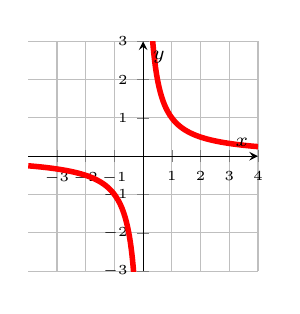
\begin{tikzpicture}[]
	\begin{axis}[width=4.5cm,height=4.5cm, axis background/.style={fill=white}, axis lines=middle, 
	grid = major,
	xlabel=$\scriptstyle x$,
	ylabel=$\scriptstyle y$, 
	xtick={-3,-2,...,5},
	ytick={-3,-2,...,3},
	ymin = -3,
	ymax = 3,
	tick label style={font=\tiny},
	legend style={font=\footnotesize,legend pos=outer north east},]
	\addplot[red, domain=-4:-0.01, samples=201, line width=2pt]{1/x};
	\addplot[red, domain=0.01:4, samples=201, line width=2pt]{1/x};		
	\end{axis}
	\end{tikzpicture}
	\task 	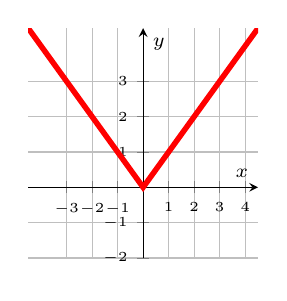
\begin{tikzpicture}[]
	\begin{axis}[width=4.5cm,height=4.5cm, axis background/.style={fill=white}, axis lines=middle, 
	grid = major,
	xlabel=$\scriptstyle x$,
	ylabel=$\scriptstyle y$, 
	xtick={-3,-2,...,5},
	ytick={-3,-2,...,3},
	ymin = -2,
	ymax = 4.5,
	tick label style={font=\tiny},
	legend style={font=\footnotesize,legend pos=outer north east},]
	\addplot[red, samples=201, line width=2pt]{abs(x)};	
	\end{axis}
	\end{tikzpicture}
\end{tasks}

 
\end{mylist}
\end{autoaval}
 
\newpage
\resum
\begin{center}
	\renewcommand{\arraystretch}{1.5}
\begin{longtable}{|p{0.2\textwidth}|p{0.35\textwidth}|p{0.3\textwidth}|} 
	\hline 
	\cellcolor{lightgray}\textbf{Punts}
	 & \vspace{-0.25cm}
	 \begin{center}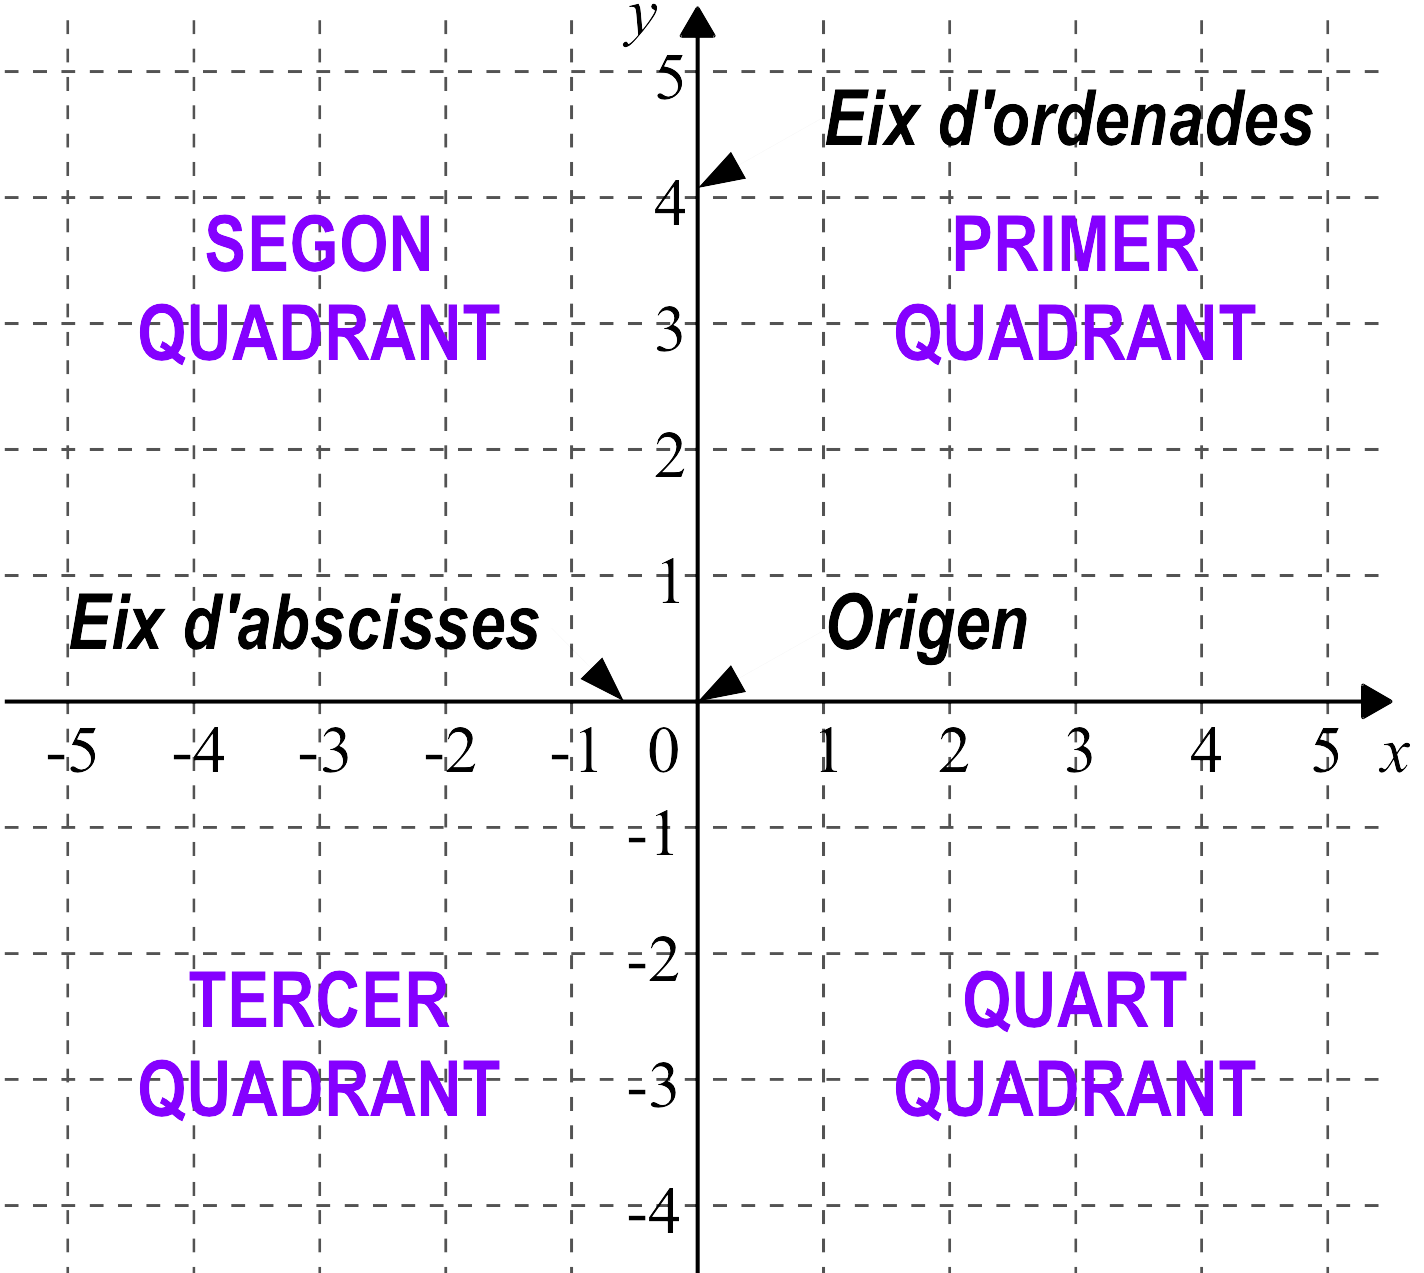
\includegraphics[width=0.32\textwidth]{img-08/image23.png}\end{center}\vspace{-0.25cm} & \vspace{-0.25cm} \begin{center}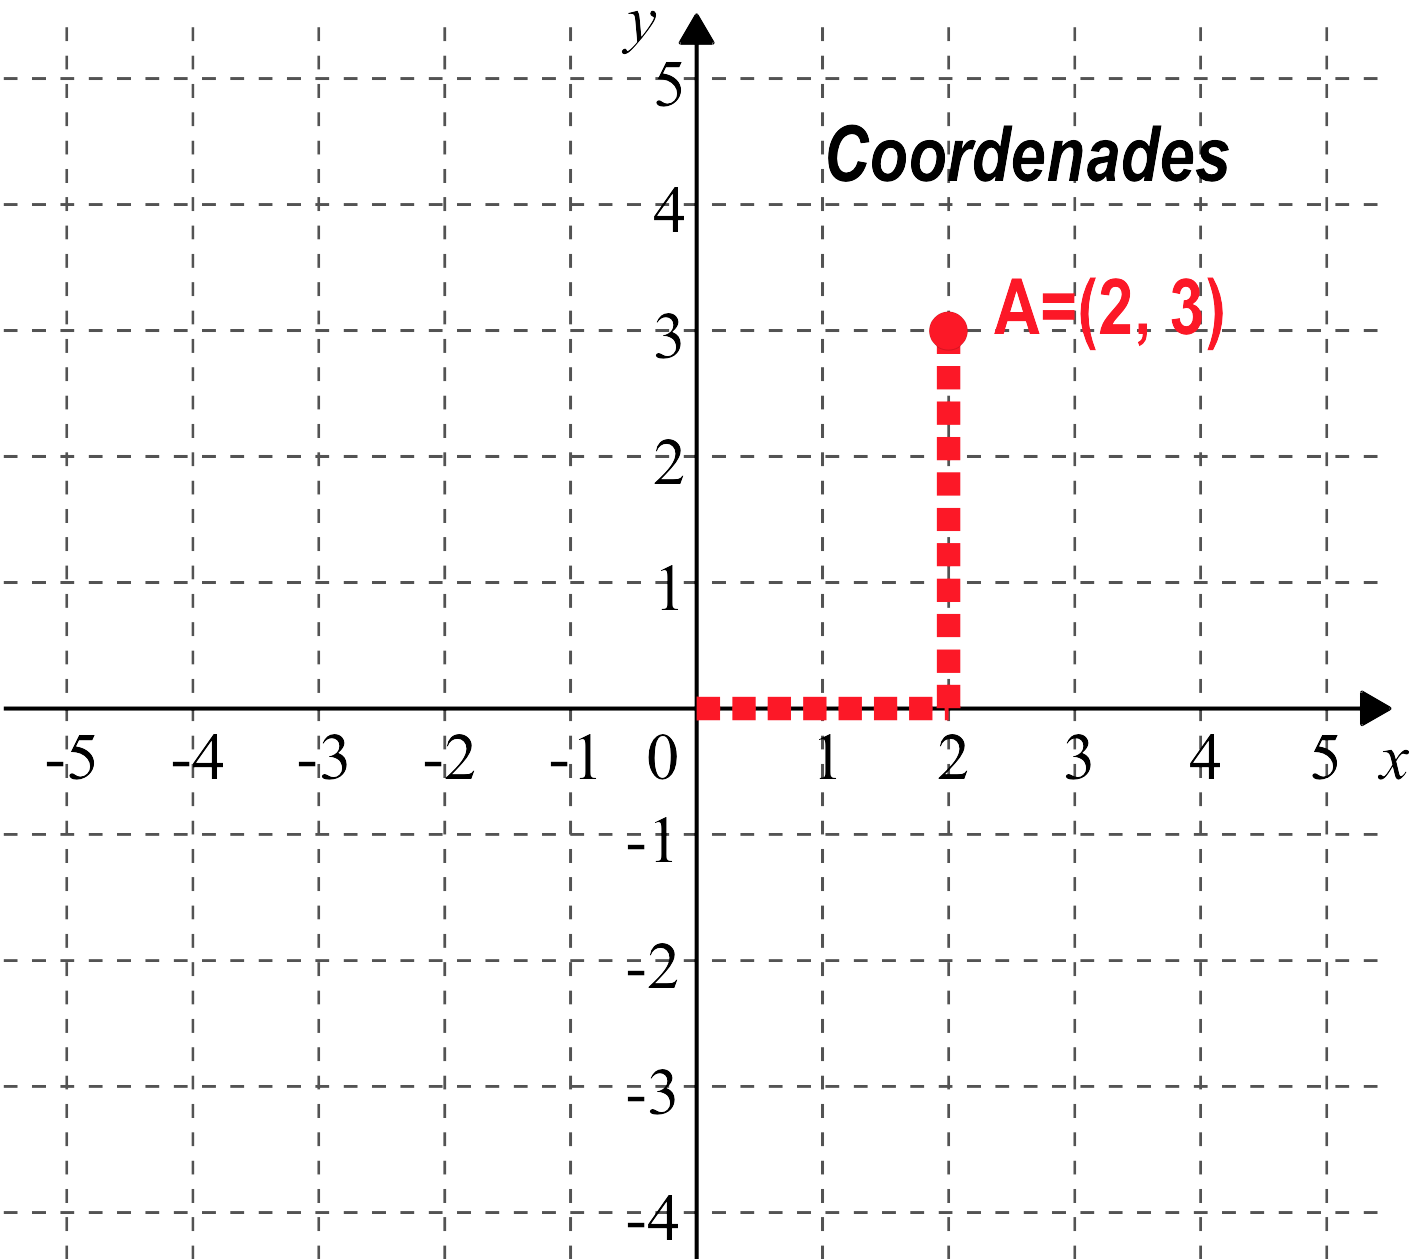
\includegraphics[width=0.32\textwidth]{img-08/image24.png}\end{center} \vspace{-0.25cm} \\ \hline
	 
	\rowcolor{lightgray} \multicolumn{3}{|p{\textwidth}|}{\textbf{Funció}} \\ \hline
 	 
\multicolumn{2}{|p{0.55\textwidth}|}{ Una \textbf{funció }és una relació entre dues magnituds de manera que a un valor qualsevol d'una (\textbf{variable independent}) li fem correspondre, com a molt, un únic valor de l'altra (\textbf{variable depenent}).} & 
\newline

$\begin{array}{l} {y=f\left(x\right)=0,59\, \cdot \, x} \\ {f\left(2\right)=0,59\, \cdot \, 2=1,18} \\ {f\left(5\right)=0,59\, \cdot \, 5=2,95} \end{array}$ \\ \hline 

	\rowcolor{lightgray} \multicolumn{3}{|p{\textwidth}|}{\textbf{Gràfica d'una funció}} \\ \hline

\multicolumn{2}{|p{0.55\textwidth}|}{ La \textbf{gràfica d'una funció }és la representació en el pla cartesià de tots els parells ordenats en els quals el primer valor correspon a un qualsevol de la variable independent i el segon al que s'obté en transformar-ho mitjançant la funció:\newline $\{$(\textit{x}, \textit{y}) $\in$ \textbf{$\Re$}, \textit{y =} \textit{f}(\textit{x})$\}$} & 
\textit{Gràfica: } 

\begin{center}
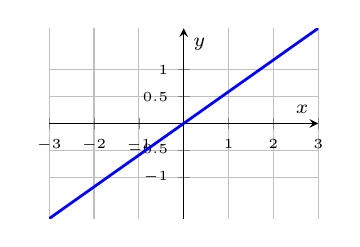
\begin{tikzpicture}[]
\begin{axis}[width=5cm,height=4cm, axis background/.style={fill=white}, axis lines=middle, 
 grid = major,
xlabel=$\scriptstyle x$,
ylabel=$\scriptstyle y$, 
xtick={-3,-2,...,3},
ytick={-1,-0.5,...,1},
tick label style={font=\tiny},
legend style={font=\footnotesize,legend pos=outer north east},]
\addplot[blue,domain=-3:3,samples=201, line width=1pt]{.59*x};	
\end{axis}
\end{tikzpicture}

$y=f(x)=0,59 x$
\end{center}
\\ \hline 

	\rowcolor{lightgray} \multicolumn{3}{|p{\textwidth}|}{\textbf{Funció afí, funció lineal i funció constant}} \\ \hline
	
 \multicolumn{2}{|p{0.55\textwidth}|}{
Una \textbf{funció afí} és aquella funció en la qual la relació entre les dues variables ve donada per un polinomi de grau menor o igual a 1: 
\[y=mx+n\]
La representació gràfica és una recta. 

``\textit{m}''\textit{ }rep el nom de \textbf{pendent} i ``\textit{n}''\textit{ }\textbf{ordenada a l'origen.}

Una \textbf{funció lineal } o \textbf{ de proporcionalitat directa} és una funció afí amb ordenada en l'origen nul·la: \textit{y = mx }(passa per l'origen).


Una \textbf{funció constant }és una funció afí amb pendent nul: \textit{y = n} (sempre pren el mateix valor i la seva gràfica és una recta horitzontal).} &
\begin{center}
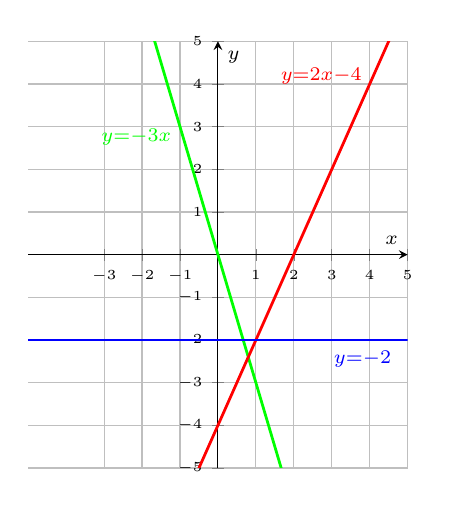
\begin{tikzpicture}
\begin{axis}[width=6.4cm,height=7cm, axis background/.style={fill=white}, axis lines=middle, 
 grid = major,
xlabel=$\scriptstyle x$,
ylabel=$\scriptstyle y$, 
xtick={-3,-2,...,5},
ytick={-5,-4,...,5},
ymin = -5,
ymax = 5,
tick label style={font=\tiny},
legend style={font=\footnotesize,legend pos=outer north east},]
\addplot[green, domain=-2:2, samples=201, line width=1pt]{-3*x} node[above, pos=1, xshift=-2cm, yshift=4.5cm] {$\scriptstyle y=-3x$};
\addplot[red, samples=201, line width=1pt]{2*x-4} node[anchor=north east,yshift=-0.75cm, xshift=-0.45cm] {$\scriptstyle y=2x-4$};
\addplot[blue, samples=201, line width=1pt]{-2} node[anchor=north east,xshift=-0.075cm] {$\scriptstyle y=-2$};	
\end{axis}
\end{tikzpicture}
\end{center}
 \\ \hline 
 
 \end{longtable}

 \pagebreak
 
 \renewcommand{\arraystretch}{2.5}
 \begin{longtable}{|p{0.2\textwidth}|p{0.35\textwidth}|p{0.3\textwidth}|} 
 	\hline 
 	\rowcolor{lightgray} \multicolumn{3}{|p{\textwidth}|}{\textbf{Funció quadràtica}} \\ \hline
 
  \multicolumn{2}{|p{0.55\textwidth}|}{Una funció quadràtica és aquella funció en la qual la relació entre les dues variables ve donada per un polinomi de grau dos:
\[y=f(x)=a x^2+b x + c\]
La gràfica d'aquest tipus de funcions es diu paràbola.

 El punt més significatiu de la paràbola és el \textbf{vèrtex} i es calcula donant-li a la variable independent el valor $x_v= -b/2a$
 
  Si el coeficient de $x^{ 2}$ és positiu, el vèrtex és un mínim i, si és negatiu, un màxim.} & 
\begin{center}
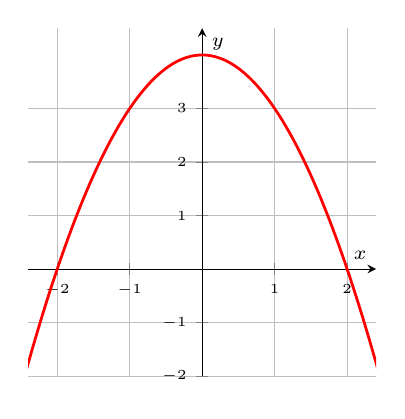
\begin{tikzpicture}[]
\begin{axis}[width=6cm,height=6cm, axis background/.style={fill=white}, axis lines=middle, 
 grid = major,
xlabel=$\scriptstyle x$,
ylabel=$\scriptstyle y$, 
xtick={-3,-2,...,5},
ytick={-3,-2,...,3},
ymin = -2,
ymax = 4.5,
tick label style={font=\tiny},
legend style={font=\footnotesize,legend pos=outer north east},]
\addplot[red, samples=201, line width=1pt]{4-x^2};	
\end{axis}
\end{tikzpicture}

$y=4-x^2$
\end{center}
 \\ 
\hline 

	\rowcolor{lightgray} \multicolumn{3}{|p{\textwidth}|}{\textbf{Continuïtat, Monotonia, Extrems, Simetria  i Periodicitat}} \\ \hline
 
  \multicolumn{2}{|p{0.55\textwidth}|}{
  Una funció pot ser:
  
  \begin{itemize}
   \item contínua en un interval si la seva gràfica no sofreix ``ruptures'' (anomenades \textbf{discontinuïtats})
   
   \item \textbf{creixent }(\textbf{decreixent}) si el seu valor augmenta (disminueix) quan ho fa la variable independent
   
   \item \textbf{constant }quan sempre pren el mateix valor
   
   \item \textbf{parell} si la imatge de la variable independent coincideix amb el del seu oposat, \textbf{imparell} quan el valor de la funció per a l'oposat de la variable independent també és l'oposat 
   
   \item \textbf{periòdica} si les imatges dels valors obtinguts en sumar una quantitat fixa (\textbf{període}) a la variable independent coincideixen.
\end{itemize}
} &
\begin{center} \includegraphics*[width=0.4\textwidth]{img-08/image28.png}
\end{center}\\ \hline 
\end{longtable}
\end{center}

